% Sandia National Laboratories is a multimission laboratory managed and
% operated by National Technology & Engineering Solutions of Sandia, LLC, a
% wholly owned subsidiary of Honeywell International Inc., for the U.S.
% Department of Energy’s National Nuclear Security Administration under
% contract DE-NA0003525.

% Copyright 2002-2021 National Technology & Engineering Solutions of Sandia,
% LLC (NTESS).



\begin{Device}\label{K_DEVICE}

\symbol
{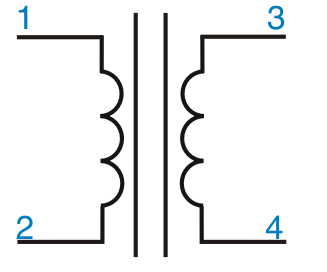
\includegraphics{transformerSymbol}}

\device
\begin{alltt}
K<name> L<inductor name> [L<inductor name>*]
+ <coupling value> [model name]
\end{alltt}

\model
.MODEL <model name> CORE [model parameters]

\examples
\begin{alltt}
ktran1 l1 l2 l3 1.0
KTUNED L3OUT  L4IN .8
KTRNSFRM LPRIMARY LSECNDRY 1
KXFRM L1 L2  L3  L4 .98 KPOT\_3C8
\end{alltt}

\parameters
\begin{Parameters}

\param{inductor name}

Identifies the inductors to be coupled. The inductors are coupled and in
the dot notation the dot is placed on the first node of each
inductor. The polarity is determined by the order of the nodes in the L
devices and not by the order of the inductors in the K statement.

If more than two inductors are given on a single K line, each inductor
is coupled to all of the others using the same coupling value.

\param{coupling value}

The coefficient of mutual coupling, which must be between $-1.0$ and
$1.0$.

This coefficient is defined by the equation
\begin{quote}
  \texttt{<coupling value>} = $\frac{M_{ij}}{\sqrt{L_iL_j}}$
\end {quote}

where
\begin{quote}
  $L_i$ is the inductance of the $i$th named inductor in the K-line
\end {quote}
\begin{quote}
    $M_{ij}$ is the mutual inductance between $L_i$ and $L_j$
\end {quote}
For transformers of normal geometry, use $1.0$ as the value. Values less
than $1.0$ occur in air core transformers when the coils do not
completely overlap.

\param{model name}

If \texttt{model name} is present, four things change:
\begin{itemize}
  \item The mutual coupling inductor becomes a nonlinear, magnetic core device.
  \item The inductors become windings, so the number specifying inductance now
        specifies the number of turns.
  \item The list of coupled inductors could be just one inductor.
  \item If two or more inductors are listed, each inductor is coupled to all others through the magnetic core.
  \item A model statement is required to specify the model parameters.
\end{itemize}

\end{Parameters}

\comments
Lead currents and power calculations are supported for the component inductors in both
linear and nonlinear mutual inductors.  They are not supported for the composite
mutual inductor though.  So, if \texttt{L1} is a component inductor for mutual inductor
\texttt{K1}, then requests for \texttt{I(L1)}, \texttt{P(L1)} and \texttt{W(L1)} will 
return lead current and power values as defined in Section~\ref{L_DEVICE}.  However, 
any usage of \texttt{I(K1)}, \texttt{P(K1)} and \texttt{W(K1)} will result in a 
\Xyce{} netlist parsing error.

\end{Device}

\paragraph{Model Parameters}
% This table was generated by Xyce:
%   Xyce -doc Min 1
%
\index{nonlinear mutual inductor!device model parameters}
\begin{DeviceParamTableGenerated}{Nonlinear Mutual Inductor Device Model Parameters}{Min_1_Device_Model_Params}
A & Thermal energy parameter & A/m & 1000 \\ \hline
ALPHA & Domain coupling parameter & -- & 5e-05 \\ \hline
AREA & Mean magnetic cross-sectional area & cm$^{2}$ & 0.1 \\ \hline
BETAH & Modeling constant & -- & 0.0001 \\ \hline
BETAM & Modeling constant & -- & 3.125e-05 \\ \hline
BHSIUNITS & Flag to report B and H in SI units & -- & 0 \\ \hline
C & Domain flexing parameter & -- & 0.2 \\ \hline
CLIM & Value below which domain flexing parameter will be treated as zero. & -- & 0.005 \\ \hline
CONSTDELVSCALING & Use constant scaling factor to smooth voltage difference over first inductor & V & false \\ \hline
DELVSCALING & Smoothing coefficient for voltage difference over first inductor & V & 1000 \\ \hline
FACTORMS & Flag to save state variables & -- & 0 \\ \hline
GAP & Effective air gap & cm & 0 \\ \hline
INCLUDEMEQU & Flag to include the magnetics in the solution. & -- & true \\ \hline
K & Domain anisotropy parameter & A/m & 500 \\ \hline
KIRR & Domain anisotropy parameter & A/m & 500 \\ \hline
LEVEL & for pspice compatibility -- ignored & -- & 0 \\ \hline
MEQNSCALING & M-equation scaling & -- & 1 \\ \hline
MS & Saturation magnetization & A/m & 1e+06 \\ \hline
MVARSCALING & M-variable scaling. & -- & 1 \\ \hline
OUTPUTSTATEVARS & Flag to save state variables & -- & 0 \\ \hline
PACK & for pspice compatibility -- ignored & -- & 0 \\ \hline
PATH & Total mean magnetic path & cm & 1 \\ \hline
PZEROTOL & Tolerance for nonlinear zero crossing & -- & 0.1 \\ \hline
REQNSCALING & R-equation scaling & -- & 1 \\ \hline
RVARSCALING & R-variable scaling & -- & 1 \\ \hline
TC1 & First order temperature coeff. & -- & 0 \\ \hline
TC2 & Second order temperature coeff. & -- & 0 \\ \hline
TNOM & Reference temperature & $^\circ$C & 27 \\ \hline
\end{DeviceParamTableGenerated}


Note that \Xyce's default value for the $\mbox{GAP}$ parameter as zero.  Some simulators
will use non-zero values of the $\mbox{GAP}$ as a default.  When using netlists from 
other simulators in \Xyce, ensure that the default parameters are consistent. 

\subparagraph{Special Notes}

The coupling coefficient of the linear mutual
inductor (i.e. a mutual inductor without a core model) is permitted to
be a time- or solution variable-dependent expression.  This is
intended to allow simulation of electromechnical devices in which
there might be moving coils that interact with fixed coils.  

Additionally, for linear mutual inductors,
different coupling terms can be applied to different pairs of inductors with this syntax:
{\tt 
\begin{verbatim}
L1 1 2 2.0e-3
L2 0 3 8.1e-3
L3 3 4 8.1e-3 
ktran1 l1 l2 0.7
ktran2 l2 l3 0.9
ktran3 l1 l3 0.99
\end{verbatim}
}

Nonlinear mutual inductors can output $B(t)$ and $H(t)$ variables so that
one can plot $B-H$ loops.  On the {\tt .print} line the $B$ and $H$ variables 
are accessible using the node output syntax as in {\tt n( non-linear-inductor-name\_b )} for $B$
and {\tt n( non-linear-inductor-name\_h )} for $H$.  A confusing aspect of this is that 
the non-linear inductor name is the {\em internal } name used by \Xyce{}.  For example, 
consider this circuit which defines a nonlinear mutual inductor at both the top level of
the circuit and within a subcircuit:

{\tt 
\begin{verbatim}
* Test Circuit for Mutually Coupled Inductors

VS 0 1 SIN(0 169.7 60HZ)
R1 1 2 1K
R2 3 0 1K
L1 2 0 10
L2 3 0 20
K1 L1 L2 0.75 txmod
.model txmod core 

.subckt mysub n1 n2 n3 
r1s n1 n2 1000
r2s n3 0  1000
L1s n2 0  10
L2s n3 0  20   
k1s L1s L2s 0.75 txmod
.ends

xtxs 1 4 5 mysub

.TRAN 100US 25MS

* output the current through each inductor and the B & H values.
.PRINT TRAN I(L1) I(L2) n(ymin!k1_b)  n(ymin!k1_h)  
+ I(xtxs:L1s)  I(xtxs:l2s) n(xtxs:ymin!k1s_b) n(xtxs:ymin!k1s_h)

.END
\end{verbatim}
}

The internal, \Xyce{} name of the non-linear mutual inductor is {\tt
YMIN!K1} or {\tt ymin!k1} as the name is not
case-sensitive.  The device {\tt k1s} is declared within a
subcircuit called {\tt xtxs}. Thus, its full name is {\tt
xtxs:ymin!k1s}. The reason for this is that both the linear and
non-linear mutual inductors are devices that are collections of other
devices, inductors in this case.  Rather than use one of the few
remaining single characters left to signify a new device, \Xyce{} uses
{\tt Y} devices as an indicator of a extended device set, where the
characters after the {\tt Y} denote the device type and then the device
name.  Here, {\tt ymin } means a {\tt min } device which is a {\em
mutual-inductor, non-linear} device.  Thus, to print the $B$ or $H$
variable of the non-linear mutual inductor called {\tt k1} one would
use {\tt n(ymin!k1\_b)} and {\tt n(ymin!k1\_h)}
respectively for a {\tt .print} line that looks like this:

{\tt 
\begin{verbatim}
.PRINT TRAN I(L1) I(L2) n(ymin!k1_b)  n(ymin!k1_h)  
\end{verbatim}
}

And if the mutual inductor is in a subcircuit called {\tt xtxs} then the 
{\tt .print} line would look like this:

{\tt 
\begin{verbatim}
.PRINT TRAN I(xtxs:L1s)  I(xtxs:l2s) n(xtxs:ymin!k1s_b) n(xtxs:ymin!k1s_h)
\end{verbatim}
}

The above example also demonstrates how one outputs the current through inductors 
that are part of mutual inductors.  
The syntax is {\tt I( inductor name )}.

Note that while MKS units are used internally in \Xyce{}, $B$ and $H$ are output
by default in the SI units of Gauss for $B$ and Oersted for $H$.
To convert $B$ to units of Tesla divide  \Xyce{}'s output by $10,000$.  
To convert $H$ to units of $A/m$ divide  \Xyce{}'s output by $4\pi/1000$. 
Additionally, one can set the {\tt .model CORE }
parameter {\tt BHSIUNITS } to 1 to force $B$ and $H$ to be output in MKS
units. 


Finally, one can access the $B$ and $H$ data via the {\tt .model
CORE} line. On the nonlinear mutual inductor's {\tt .model} line, set the
option {\tt OUTPUTSTATEVARS=1}. This will cause \Xyce{} to create a unique
file for each nonlinear mutual inductor that uses this {\tt .model} line
with a name of the form {\tt Inductor\_}device\_name.  There are five
columns of data in this file: time ($t$), magnetic moment ($M$), total
current flux ($R$), flux density ($B$) and magnetic field strength
($H$).  As with data output on the {\tt .print} line, SI units are used
such that $B$ is output with units of Gauss and $H$ in Oersted.  As
mentioned earlier, setting the model flag {\tt BHSIUNITS } to 1 causes
the output of $B$ and $H$ uses MKS units of Tesla and $A/m$
respectively. 

\index{mutualinductor!mutual inductor equations}
\subparagraph{Mutual Inductor Equations}

The voltage to current relationship for a set of linearly coupled inductors is:
\begin{equation}
V_{i} = \sum_{j=1}^{N} c_{ij} \sqrt{ L_{i} L_{j} } \frac{dI_{j}}{dt}
\label{linMIRelation}
\end{equation}

Here, $V_{i}$ is the voltage drop across the $i$th inductor in the coupled set.
The coupling coefficient between a pair of inductors is $c_{ij}$ with a value typically
near unity and $L$ is the inductance of a given inductor which has units of
\emph{Henry's} (1 Henry $ = 1 H = Volt \cdot s / Amp $)

For nonlinearly coupled inductors, the above equation is expanded to the form:
\begin{equation}
V_{i} = \left[1 + \left(1-\frac{\ell_g}{\ell_t}\right)P(M,I_{1} ... I_{N})\right]\sum_{j=1}^{N} Lo_{ij} \frac{dI_{j}}{dt}
\label{nonlinMIRelation}
\end{equation}
This is similar in form to the linearly coupled inductor equation.  However,
the coupling has become more complicated as it now depends on the magnetic moment
created by the current flow, $M$.  Additionally, there are geometric factors,
$\ell_{g}$ and $\ell_{t}$ which are the effective air gap and total mean magnetic
path for the coupled inductors. The matrix of terms, $Lo_{ij}$ is defined as
\begin{equation}
Lo_{ij}=\frac{\mu_0 A_c N_i N_j}{\ell_t}
\end{equation}
and it represents the physical coupling between inductors $i$ and $j$.  In this
expression, $N_i$ is the number of windings around the core of inductor $i$,
$\mu_0$ is the magnetic permeability of free space which has units of Henries per meter
and a value of $4\pi \times 10^{-7}$ and $A_c$ is the mean magnetic cross-sectional area.

The magnetic moment, $M$ is defined by:
\begin{equation}
\frac{dM}{dt} = \frac{1}{\ell_t} P \sum_{i=1}^{N} N_i \frac{dI_i}{dt}
\end{equation}
and the function $P$ is defined as:
\begin{equation}
P = \frac{c M'_{an} + (1-c)M'_{irr}}{1 + \left(\frac{\ell_g}{\ell_t}-\alpha\right) c M'_{an} + \frac{\ell_g}{\ell_t}(1-c)M'_{irr}}
\end{equation}
If $c < \mbox{CLIM}$, then $c$ is treated as zero in the above equation and \Xyce\/ 
simplifies the formulation.  In this case, the magnetic-moment equation will not be 
needed and it will be be dropped form the formulation.  One can controll this behavior by
modifying the value of $\mbox{CLIM}$.

The remaining functions are:
\begin{eqnarray}
M'_{an} & = & \frac{M_s A}{\left(A + |H_e|\right)^2} \\
H_e & = & H + \alpha M \\
H & = & H_{app} - \frac{\ell_g}{\ell_t}M  \\
H_{app} & = & \frac{1}{\ell_t}\sum_{i=1}^{N} N_i I_i \\
M'_{irr} & = & \frac{\Delta M sgn(q) + |\Delta M|}{2\left(K_{irr} - \alpha |\Delta  M|\right)} \\
\Delta M & = & M_{an} - M \\
M_{an} & = & \frac{M_s H_e}{A + |H_e|} \\
q & = & \mbox{DELVSCALING}  \Delta V
\end{eqnarray}

\Xyce\/ dynamically modifies $\mbox{DELVSCALING}$ to be $1000 / $ Maximum Voltage Drop over the 
first inductor.  This typically produces accurate results for both low voltage and high 
voltage applicaitons.  However, it is possible to use a fixed scaling by setting the 
model parameter $\mbox{CONSTDELVSCALING}$ to true and then setting $\mbox{DELVSCALING}$ 
to the desired scaling value.

In \Xyce{}'s formulation, we define $R$ as:
\begin{equation}
R = \frac{dH_{app}}{dt} = \frac{1}{\ell_t}\sum_{i=1}^{N} N_i \frac{dI_i}{dt}
\end{equation}
This simplifies the $M$ equation to:
\begin{equation}
\frac{dM}{dt} =  P R
\end{equation}
\Xyce{} then solves for the additional variables $M$ and $R$ when modeling a nonlinear
mutual inductor device.

\subparagraph{B-H Loop Calculations}
\index{mutualinductor!B-H loop calculations}
To calculate $B$-$H$ loops, $H$ is used as defined above and $B$ is a derived quantity
calculated by:
\begin{eqnarray}
B & = & \mu_0 \left( H + M \right) \\
  & = & \mu_0 \left[ H_{app} + \left(1 - \frac{\ell_g}{\ell_t}\right) M \right]
\end{eqnarray}

\subparagraph{Converting Nonlinear to Linear Inductor Models} 
\index{mutualinductor!Converting nonlinear to linear mutual indcutors}
At times one may have a model for nonlinear mutual inductor, but wish to use a 
simpler linear model in a given circuit.  To convert a non-linear model to an 
equivalent linear form, one can start by equating the coupling components of 
equations~\ref{linMIRelation} and~\ref{nonlinMIRelation} as:

\begin{equation}
 c_{ij} \sqrt{ L_{i} L_{j} } =  \left[1 + \left(1-\frac{\ell_g}{\ell_t}\right)P(M,I_{1} ... I_{N})\right] Lo_{ij}
\label{nonlinMIRelation2}
\end{equation}
In the above relationship, $i$ and $j$ represent the $i$th and $j$th inductors.  Since we would like to 
equate the $i$th inductor's nonliner properties to its linear properties, we will substitute $i\rightarrow j$ 
and simplify assuming steady state where $d/dt = 0$ and $M(t) = 0$.

\begin{equation}
L_{i} = \frac{1}{c_{ii}} \left\{ 1 + \left(1 - \frac{\ell_g}{\ell_t}  \right) 
  \left[\frac{c \frac{Ms}{A}}{1 + \left( \frac{\ell_g}{\ell_t} - \alpha\right) \frac{Ms}{A}} \right] \right\} \frac{\mu A_c}{\ell_t} N_i^2
  \label{inductanceFromWindings}
\end{equation}

In the above equatin, $c_{ii}$ represents the coupling coefficient between the $i$th inductor with itself.  
This will likely be $1$ unless there are very unusual geometry considerations.  Note, that the terms $A$, $Ms$, $A_c$, $\mu$,
$\ell_{g}$ and $\ell_{t}$ all have units of length within them and must use the same unit for this relationship 
to be valid.  Specifically, $\mu$ has units of Henery's per meter and $A$ and $Ms$ have units of Amps per meter.   
$A_c$, $\ell_{g}$ and $\ell_{p}$ have units of length$^2$ and length respectively, but the length unit used in 
the model statement is $cm^2$ and $cm$ respectively.  Thus, one must use consistent units such as meters 
for $A_c$, $\ell_{g}$ and $\ell_{p}$ in equation~\ref{inductanceFromWindings} for a valid inductance approximation.

